\documentclass{standalone}
\usepackage[utf8]{inputenc}
\usepackage[T1]{fontenc}
\usepackage{graphicx}
\usepackage{amsmath}
\usepackage[american,siunitx]{circuitikz}
\usetikzlibrary{arrows,shapes,calc,positioning}
\usepackage{tikzsymbols}
\usepackage{gensymb}


\begin{document}
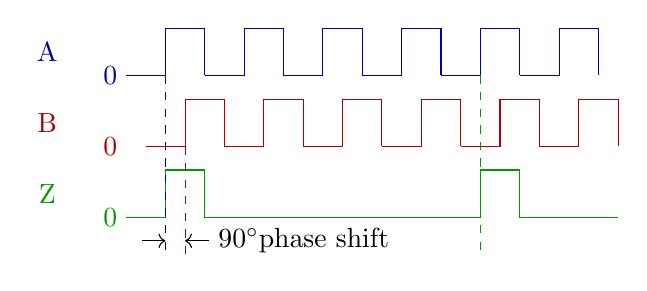
\begin{tikzpicture}[yscale=0.6,]
  \begin{scope}
    \def\clr{blue!70!black}
    \node[\clr] at (0, 0.5) {A};
    \node[\clr] at (0.8, 0) {0};
    \foreach \x in {1, 2, 3,...,6} {
      \pgfmathsetmacro{\mid}{\x + 0.5}
      \pgfmathsetmacro{\endd}{\x + 1}
      \draw[\clr] (\x, 0) -- (\mid, 0) -- (\mid, 1) -- (\endd, 1) -- (\endd, 0);
      }
  \end{scope}
\begin{scope}[yshift=-15mm,]
    \def\clr{red!70!black}
    \node[\clr] at (0, 0.5) {B};
    \node[\clr] at (0.8, 0) {0};
    \foreach \x in {1.25, 2.25, 3.25,...,6.25} {
      \pgfmathsetmacro{\mid}{\x + 0.5}
      \pgfmathsetmacro{\endd}{\x + 1}
      \draw[\clr] (\x, 0) -- (\mid, 0) -- (\mid, 1) -- (\endd, 1) -- (\endd, 0);
      }
  \end{scope}
  
  \begin{scope}[yshift=-30mm,]
    \def\clr{green!60!black}
    \node[\clr] at (0, 0.5) {Z};
    \node[\clr] at (0.8, 0) {0};
    \draw[\clr] (1, 0) -- (1.5, 0) -- (1.5, 1) -- (2, 1) -- (2, 0)
    -- (5.5, 0) -- (5.5, 1) -- (6, 1) -- (6, 0) -- (7.25, 0);
  \end{scope}


  \draw[dashed, blue!70!black] (1.5, 0) -- (1.5, -3.8);
  \draw[dashed, red!70!black] (1.75, -1.5) -- (1.75, -3.8);

  \draw[->] (1.2, -3.5) -- (1.5, -3.5);
  \draw[<-] (1.75, -3.5) -- (2.05, -3.5) node[right] {90\degree phase shift};


  \draw[dashed, green!60!black] (5.5, 0) -- (5.5, -3.8);

\end{tikzpicture}
\end{document}
